
%% ==================================================================================================
%%
\documentclass[12pt]{book}
\usepackage{amsfonts}
\usepackage{amsmath}
\usepackage{amssymb}
\usepackage{graphicx}
\usepackage{hyperref}
\usepackage{float}
\usepackage{verbatim}
\usepackage{xlop} %% for multiplication https://tex.stackexchange.com/questions/11702/how-to-present-a-vertical-multiplication-addition
\usepackage{listings} %% to format generic computer code
\usepackage{lmodern} % for bold teletype font
\usepackage{minted} % colour Java code

\usepackage{tasks}
%\NewTasks[style=enumerate,counter-format=tsk[A].,label-width=3ex]{choice}[\item](4)

%% =======   set page margins    =======
\setlength{\textheight}{10in}
\setlength{\textwidth}{7.4in}
\setlength{\topmargin}{-0.75in}
\setlength{\oddsidemargin}{-0.5in}
\setlength{\evensidemargin}{-0.5in}
\setlength{\parskip}{0.15in}
\setlength{\parindent}{0in}

%%  for European long division
% https://tex.stackexchange.com/questions/432435/how-to-set-up-european-french-style-long-division-in-tex
\newcommand\frdiv[5]{%
    \[
    \renewcommand\arraystretch{1.5}
    \begin{array}{l| l}
    #1 & #2 \\
    \cline{2-2}
    #3 & #4 \\
    \cline{1-1}
    #5 & \\
    \end{array}
    \]
}

%%  for European long division


%% ==================================================================================================

\begin{document}

%\title{ITI1100 Digital Systems I}
%\author{Kien Do 300163370}
%\date{Assignment \#1}
\newcommand{\reporttitle}{Devoir 7}
\newcommand{\reportauthorOne}{Kien Do}
\newcommand{\cidOne}{300163370}
\input{titlePage/titlepage.txt}



%% ==================================================================================================

%%%%%%%%%%%% PROBLEMS START HERE
\begin{enumerate}
    
    \item
    
    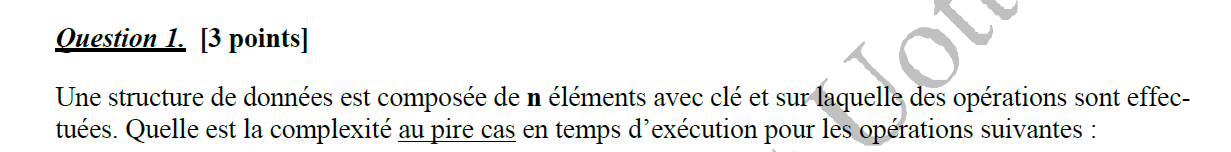
\includegraphics[scale=0.69]{d7q1q.png}\\
    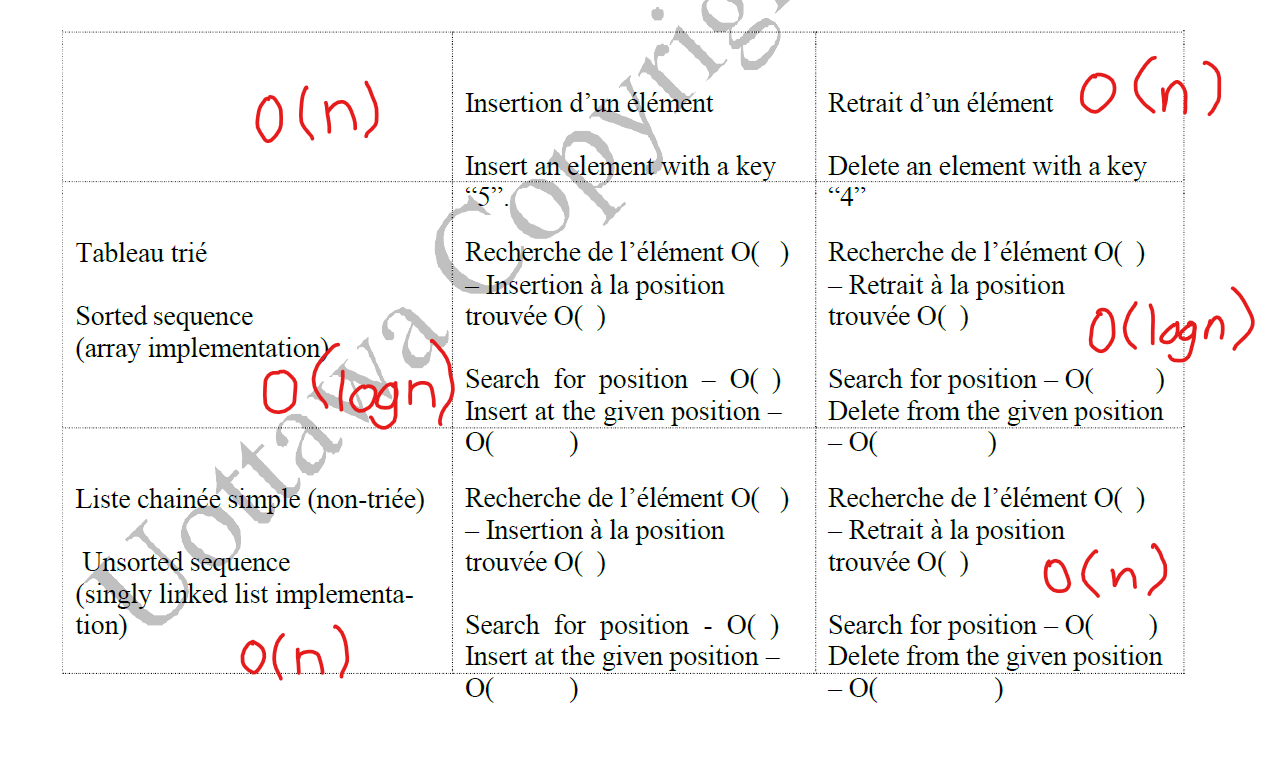
\includegraphics[scale=0.69]{d7q1a1.png}\\
    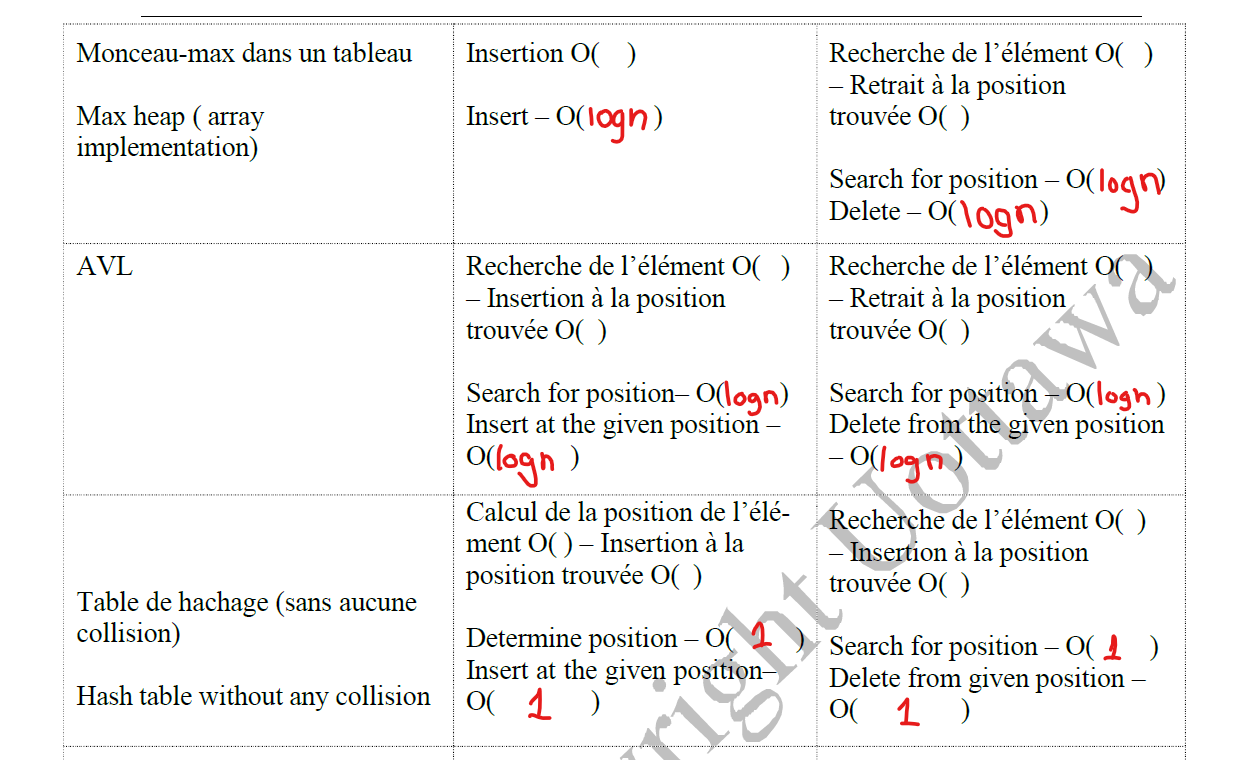
\includegraphics[scale=0.69]{d7q1a2.png}\\
    
    \newpage
    
    \item 
    
    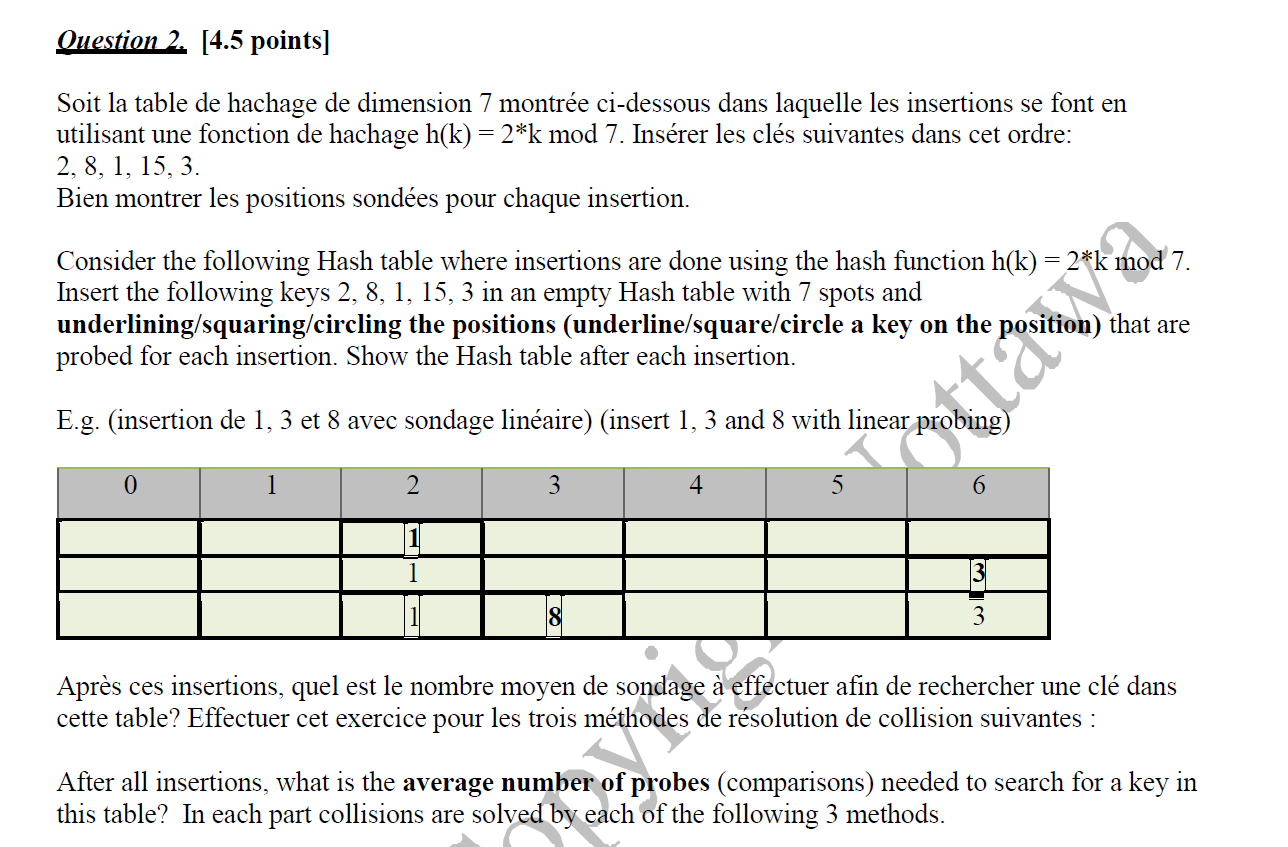
\includegraphics[scale=0.7]{d7q2q1.png}\\
    
    a) Sondage linéaire. Linear probing.\\
    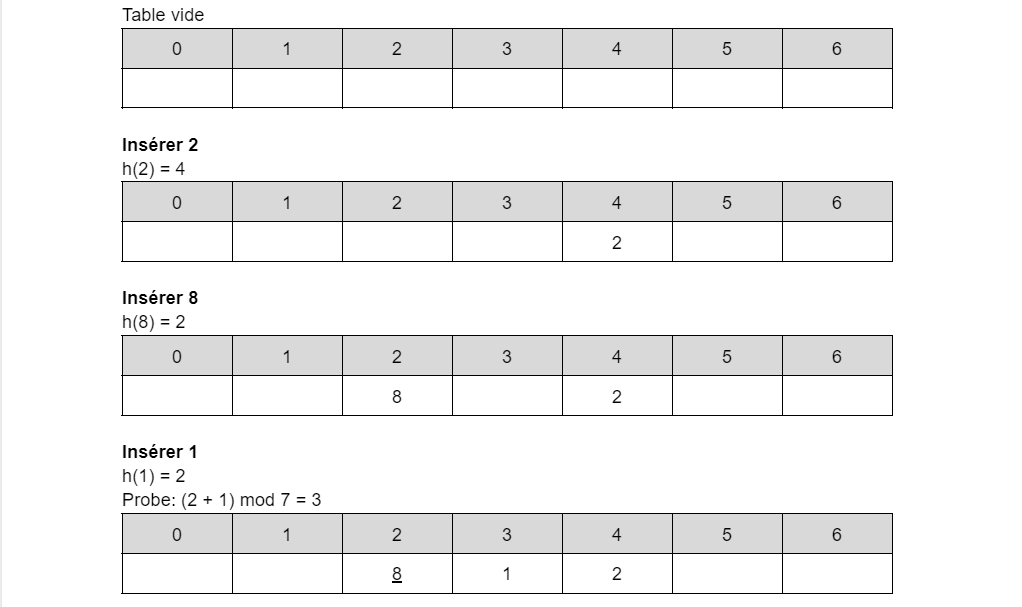
\includegraphics[scale=0.7]{d7q2a1a.png}\\
    \newpage
    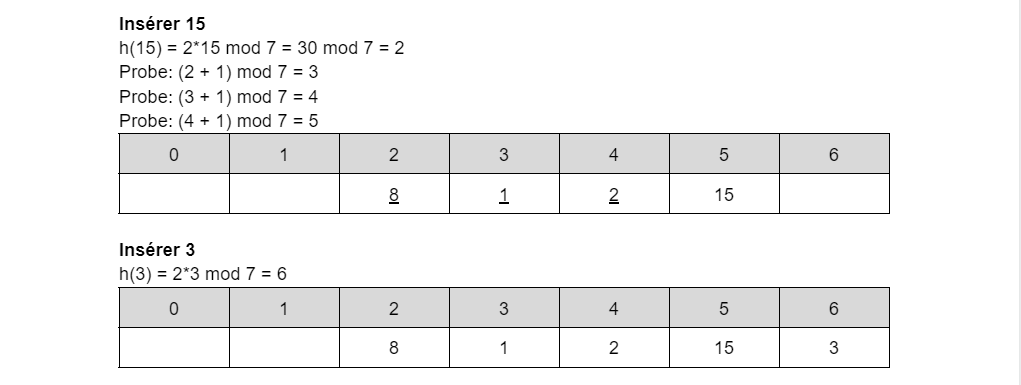
\includegraphics[scale=0.7]{d7q2a1b.png}\\
    Nombre moyen de sondages = (0 + 0 + 1 + 3 + 0)/5 = 0.8 probes.\\
    
    b) Sondage quadratique. Quadratic probing.\\
    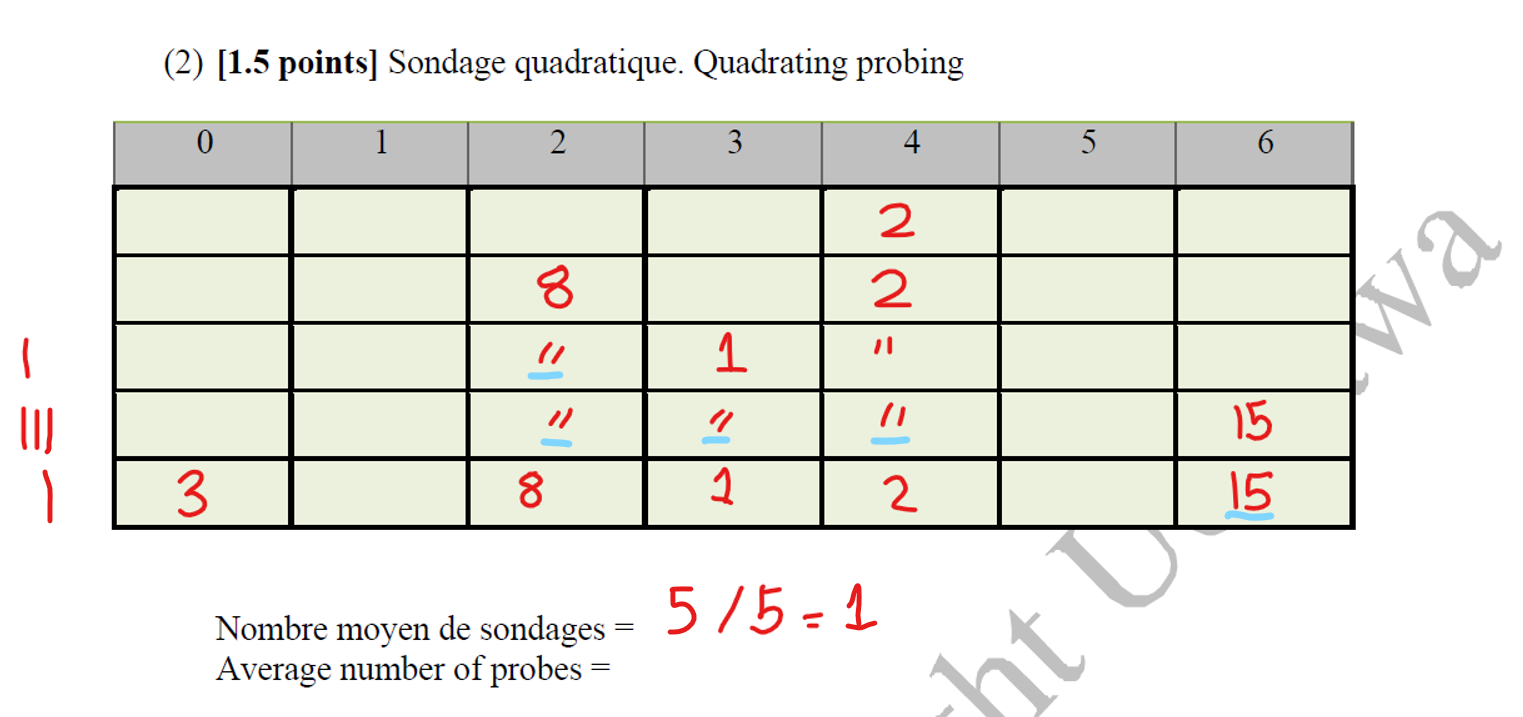
\includegraphics[scale=0.40]{d7q2a2.png}
    
    c) Hachage double.\\
    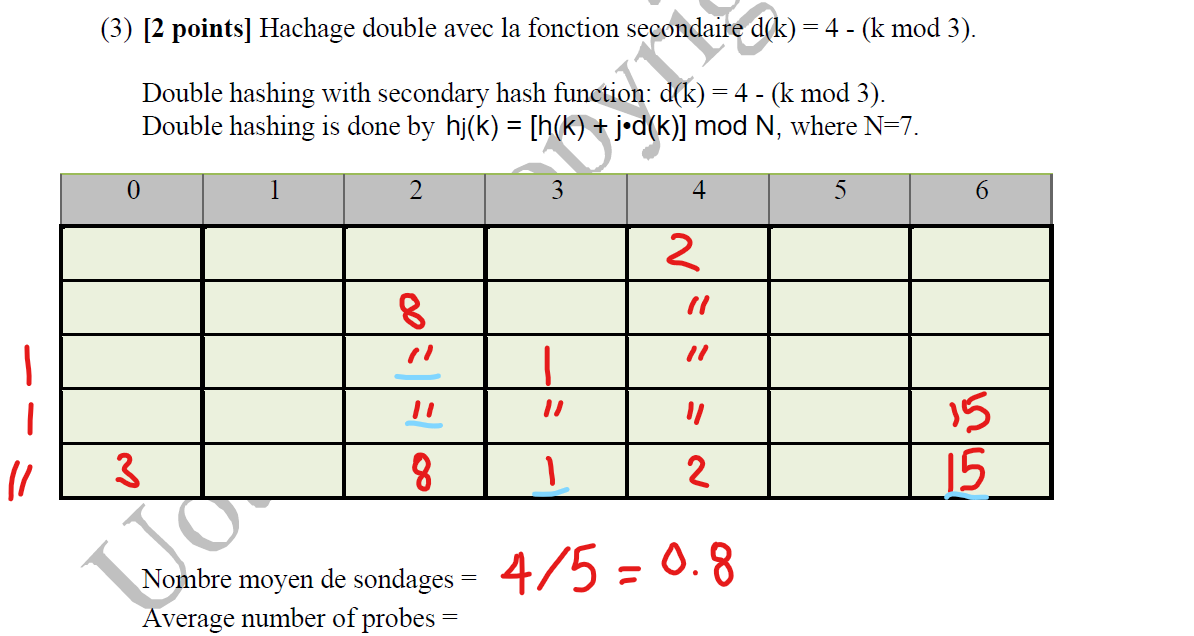
\includegraphics[scale=0.5]{d7q2a3.png}
    \newpage
    
    \item 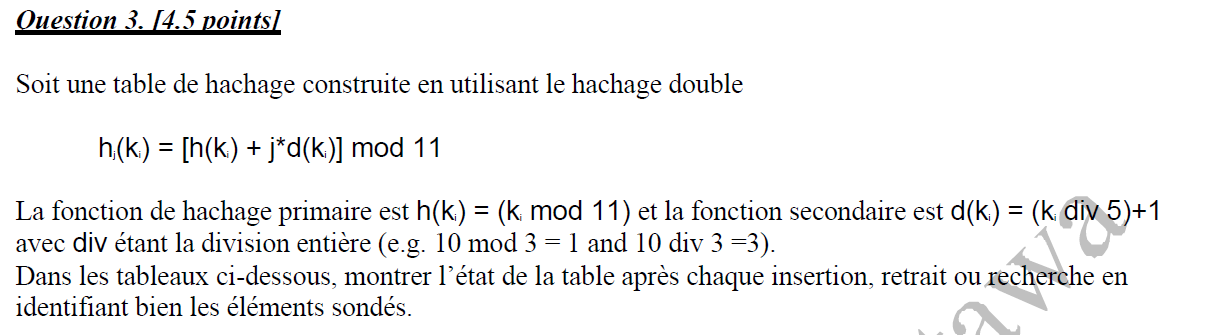
\includegraphics[scale=0.50]{d7q3q.png}\\
    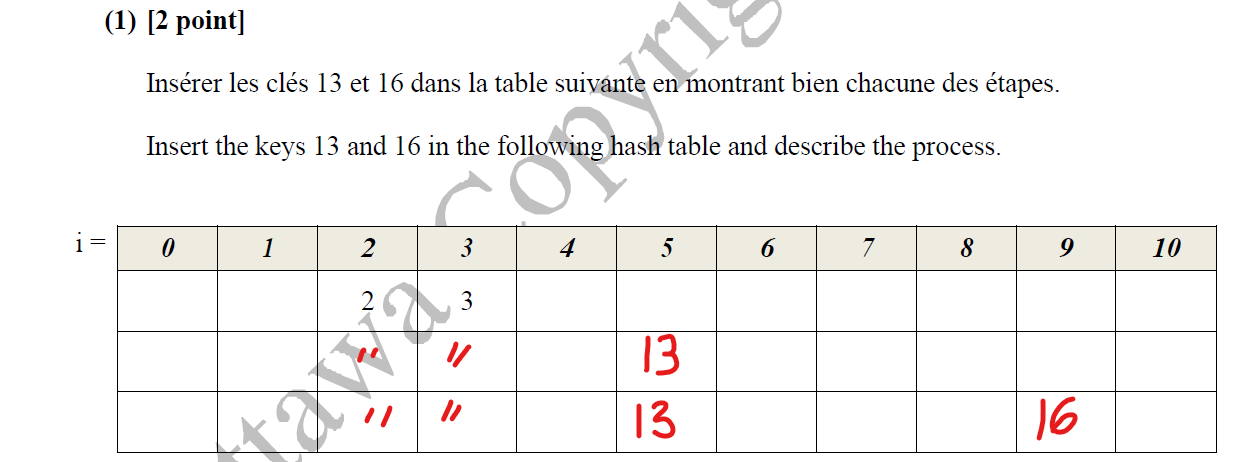
\includegraphics[scale=0.60]{d7q3a1.png}
    
    \textbf{Description:}\\
    Insertion de la clé 13.
    \begin{align*}
        h(13) &= 13 \mod 11 = 2 \qquad \xleftarrow[]{\text{déjà occupé par 2}}\\
        d(13) &= (13 \text{ div } 5) + 1 = 2 + 1 = 3\\
        (j = 1) \quad &[2 + (1)(3)]\mod 11 = 5 \qquad \xleftarrow[\text{faire l'insertion à i = 5}]{\text{disponible}}
    \end{align*}
    
    Insertion de la clé 16.
    \begin{align*}
        h(16) &= 16 \mod 11 = 5 \qquad \xleftarrow[]{\text{déjà occupé par 13}}\\
        d(16) &= (16 \text{ div } 5) + 1 = 3 + 1 = 4\\
        (j = 1) \quad &[5 + (1)(4)]\mod 11 = 9 \qquad \xleftarrow[\text{faire l'insertion à i = 9}]{\text{disponible}}
    \end{align*}
    
    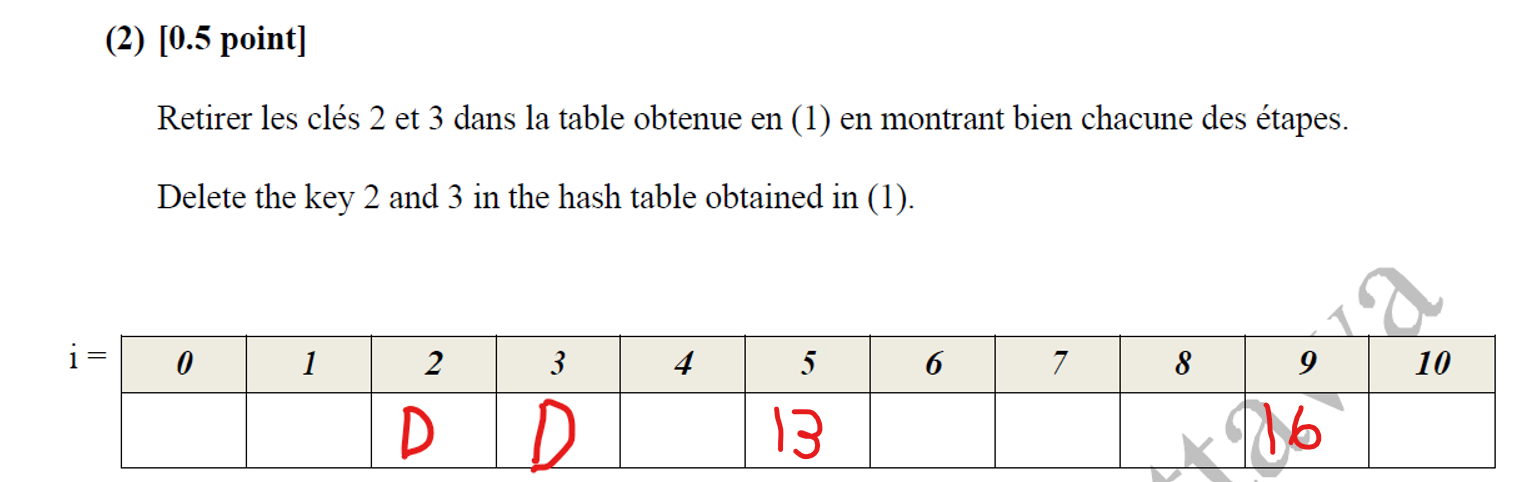
\includegraphics[scale=0.50]{d7q3a2.png}
    
    \textbf{Description:}\\
    Retirer la clé 2 (on fait la même chose avec la clé 3).
    \begin{align*}
        h(2) &= 2 \mod 11 = 2 \qquad \xleftarrow[\text{remplace avec la clé D (disponible)}]{\text{clé est trouvé}}\\
    \end{align*}
    
    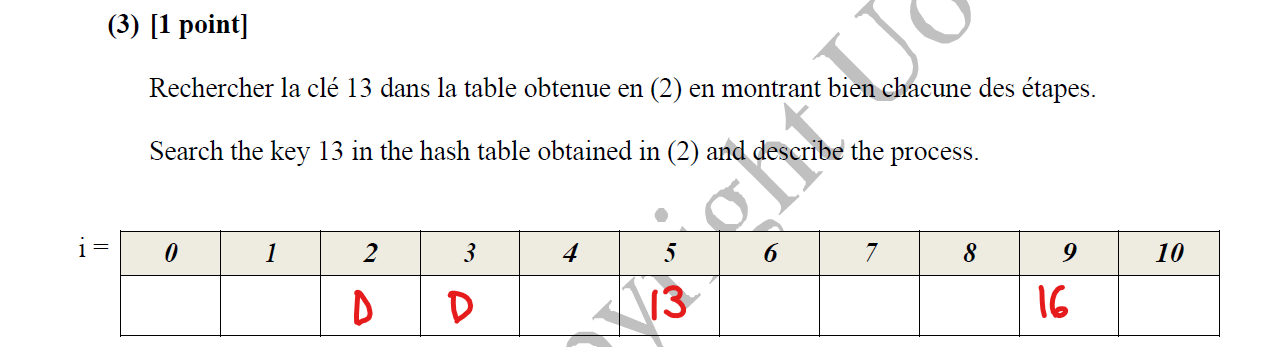
\includegraphics[scale=0.60]{d7q3a3.png}\\
    Rechercher la clé 13.
    \begin{align*}
        h(13) &= 13 \mod 11 = 2 \qquad \xleftarrow[]{D \neq 13}\\
        d(13) &= (13 \text{ div } 5) + 1 = 2 + 1 = 3\\
        (j = 1) \quad &[2 + (1)(3)]\mod 11 = 5 \qquad \xleftarrow[\text{retourne l'élément à i = 5}]{\text{13 == 13}}
    \end{align*}
    
    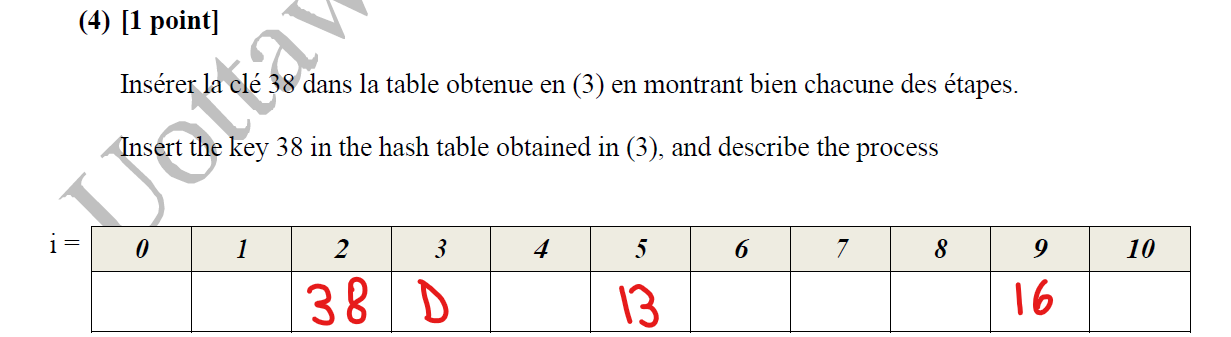
\includegraphics[scale=0.60]{d7q3a4.png}\\
    Insérer la clé 38.
    \begin{align*}
        h(38) &= 38\mod 11 = 5 \qquad \xleftarrow[]{\text{déjà occupé par 13}}\\
        d(38) &= (38 \text{ div } 5) + 1 = 3 + 1 = 4\\
        (j = 1) \quad &[5 + (1)(4)]\mod 11 = 9 \qquad \xleftarrow[\text{j++}]{\text{déjà occupé par 16}}\\
        (j = 2) \quad &[2 + (2)(4)]\mod 11 = 2 \qquad \xleftarrow[\text{remplace D avec 38}]{\text{disponible}}
    \end{align*}
    
    
    
    
\end{enumerate}





\end{document} 
